\begin{abcliste}
\abc Die Strecke ist die Fläche unter dem $v(t)$-Graphen: zwei Dreiecke und ein Rechteck.
\begin{align}
 \Delta s_1 &= \dOneF = \frac{1}{2}\cdot\vMax\cdot\tOne = \dOne \\
 \Delta s_2 &= \dTwoF = \vMax\cdot\tTwo = \dTwo \\
 \Delta s_3 &= \dThreeF = \frac{1}{2}\cdot\vMax\cdot\tThree = \dThree \\
 \Delta s &= \dsF = \ds \approx \result{\dsP{0}{3}}
\end{align}
\abc Die ganze Fahrt dauert
\begin{align}
 t_\mathrm{tot} &= \tTotF = \tTot
\end{align}
und die mittlere Geschwindigkeit ist
\begin{align}
 \bar v &= \vMeanF = \frac{\ds}{\tTot} = \vMean \approx \result{\vMeanP{0}{2}}
\end{align}
\abc Die mittlere Geschwindigkeit ist die Höhe des Rechtecks über der ganzen Fahrzeit, das dieselbe Fläche hat wie die Fläche unter dem $v(t)$-Graphen (rot gestrichelt). Mit dieser konstanten Geschwindigkeit wäre die Velofahrerin in derselben Zeit gleich weit gekommen.
\begin{center}
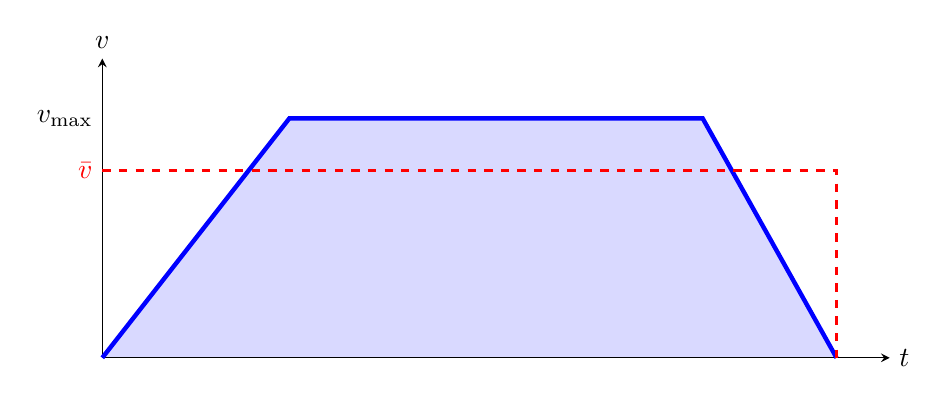
\begin{tikzpicture}[>=stealth, x=0.25cm, y=0.4cm]
 \fill[blue, opacity=0.15] (0,0) -- (9.5,7.6) -- (30.5,7.6) -- (37.3,0) -- cycle;
 \draw[->] (0,0) -- (40,0) node[right] {$t$};
 \draw[->] (0,0) -- (0,9.5) node[above] {$v$};
 \draw[ultra thick, blue] (0,0) -- (9.5,7.6) -- (30.5,7.6) -- (37.3,0);
 \draw[very thick, red, dashed] (0,5.94) -- (37.3,5.94) -- (37.3,0);
 \node[left] at (0,7.6) {$v_\mathrm{max}$};
 \node[left, red] at (0,5.94) {$\bar v$};
\end{tikzpicture}
\end{center}
\end{abcliste}
